\documentclass[]{osa-article}

%% Select the journal you're submitting to
%% oe, boe, ome, osac, osajournal
\journal{osajournal}
% Key:
% Express journals must have the correct journal selected:
% {oe} Optics Express
% {boe} Biomedical Optics Express
% {ome} Optical Material Express
% {osac} OSAC Continuum
% Other OSA journals may use:
% {osajournal} Applied Optics, Advances in Optics and Photonics, Journal of the Optical Society of America A/B, Optics Letters, Optica, Photonics Research

% Uncomment if submitting to Photonics Research.
% ONLY APPLICABLE FOR \journal{osajournal}
% \setprjcopyright

% Set the article type
\articletype{Research Article}
% Note that article type is not required for Express journals (OE, BOE, OME and OSAC)

% Talon's custom libraries
\usepackage{empheq}
\usepackage{bm}
\usepackage[normalem]{ulem}
\usepackage{booktabs}
\usepackage{upgreek}

% Talon's custom commands
\setlength\arraycolsep{1.5pt}
\let\originalleft\left
\let\originalright\right
\renewcommand{\left}{\mathopen{}\mathclose\bgroup\originalleft}
\renewcommand{\right}{\aftergroup\egroup\originalright}
\DeclareMathAlphabet{\mathcal}{OMS}{cmsy}{m}{n}
\newcommand{\tensor}[1]{\overset{\text{\tiny$\leftrightarrow$}}{\mb{#1}}}
\newcommand{\argmin}{\arg\!\min}
\newcommand{\me}{\mathrm{e}}
\providecommand{\e}[1]{\ensuremath{\times 10^{#1}}} 
\providecommand{\mb}[1]{\mathbf{#1}}
\providecommand{\msf}[1]{\mathsf{#1}}
\providecommand{\mf}[1]{\mathfrak{#1}}
\providecommand{\mc}[1]{\mathcal{#1}}
\providecommand{\ro}{\boldsymbol{\mathfrak{r}}_o}
\providecommand{\rs}{\boldsymbol{\mathfrak{r}}_s}
\newcommand{\mypar}{\parallel}
\providecommand{\ropar}{r_o^{\mypar}}
\providecommand{\roperp}{\mathbf{r}_o^{\bot}}
\providecommand{\rspar}{r_s^{\mypar}}
\providecommand{\rsperp}{\mathbf{r}_s^{\bot}}
\providecommand{\rppar}{r_p^{\mypar}}
\providecommand{\rpperp}{\mathbf{r}_p^{\bot}}
\providecommand{\so}{\mathbf{\hat{s}}_o}
\providecommand{\rp}{\mathbf{r}_p}
\providecommand{\rbm}[1]{r_b^{\text{m}}}
\providecommand{\rd}{\mathbf{r}_d}
\providecommand{\rdf}{\mathpzc{r}_d}
\providecommand{\mh}[1]{\mathbf{\hat{#1}}}
\providecommand{\mbb}[1]{\mathbb{#1}}
\providecommand{\bs}[1]{\boldsymbol{#1}}
\providecommand{\bv}{\boldsymbol{\mathfrak{v}}}
\providecommand{\bvperp}{\bs{\nu}^{\bot}}
\providecommand{\bvpar}{\nu^{\parallel}}
\providecommand{\bt}{\bs{\uptau}}
\providecommand{\btperp}{\bs{\tau}^{\bot}}
\providecommand{\btpar}{\tau^{\mypar}}
\providecommand{\bsh}[1]{\hat{\boldsymbol{#1}}}
\providecommand{\nan}{\left(\frac{\text{NA}}{n_o}\right)}
\providecommand{\lmsum}{\sum_{\ell=0}^\infty\sum_{m=-\ell}^{\ell}}
\providecommand{\intr}[1]{\int_{\mbb{R}^{#1}}}
\providecommand{\ints}[1]{\int_{\mbb{S}^{#1}}}
\providecommand{\tb}[1]{\textcolor{blue}{#1}}
\providecommand{\eqp}{\stackrel{(p)}{=}}
\providecommand{\propp}{\stackrel{(p)}{\propto}}

\providecommand{\add}[1]{{\color{blue}#1}}
% \DeclareFontFamily{OT1}{pzc}{}
% \DeclareFontShape{OT1}{pzc}{m}{it}{<-> s * [1.10] pzcmi7t}{}
% \DeclareMathAlphabet{\mathpzc}{OT1}{pzc}{m}{it}
\newcommand{\eqname}[1]{\tag*{#1}}
\newcommand*\widefbox[1]{\fbox{\hspace{1em}#1\hspace{1em}}}

\begin{document}

\title{Spatio-angular fluorescence microscopy\\ III. Three-dimensional high-aperture 4f imaging}

\author{Talon Chandler,\authormark{1,*} Hari Shroff,\authormark{2,3} Rudolf Oldenbourg,\authormark{3} and Patrick La Rivi\`ere\authormark{1,3}}

\address{\authormark{1}University of Chicago, Department of Radiology, Chicago, Illinois 60637, USA\\
  \authormark{2}Section on High Resolution Optical Imaging, National Institute of Biomedical Imaging and Bioengineering, National Institutes of Health, Bethesda, Maryland 20892, USA\\
  \authormark{3}Marine Biological Laboratory, Bell Center, Woods Hole, Massachusetts 02543, USA}

\email{\authormark{*}talonchandler@talonchandler.com} %% email address is required

\begin{abstract*}
  TODO
\end{abstract*}

\section{Introduction}
\add{Patrick: Key references for comparison are sheppard1994} \cite{sheppard1994} \add{and arnison2002} \cite{arnison2002}.\\

\noindent Skeleton literature review ahead. \\

\noindent First and second papers transfer functions for dipoles \cite{chandler2019a, chandler2019b}\\

\noindent First 3D pupil function: \cite{mccutchen1964}\\
First paraxial 3D transfer function: \cite{frieden1967}\\
First defocused transfer functions: \cite{stokseth1969}\\
Interpretation of 3D transfer function: \cite{sheppard1989}\\
First high-aperture monopole transfer function: \cite{sheppard1994}\\
Vectorial 3D transfer function: \cite{sheppard1997a, philip1999, arnison2002, schonle2002}\\
Brief mention of dipoles and vectorial 3d transfer functions \cite{sheppard1997b, schonle2002}\\

\noindent PSF of single fixed dipole radiator \cite{sheppard1997b, nov2006, sick2000, bohmer2003, patra2004, toprak2006, backer2014, khadir2019}\\
Images/PSFs of rotating dipoles: \cite{lew2013, backlund2014, backer2015, stallinga2015, backer2019}\\
Orientation induced localization biases: \cite{engelhardt2011, stallinga2012, backlund2014}\\
3D angular transfer function approaches that use the second moments instead of the spherical harmonics \cite{aguet2009a, backer2014, brasselet2011, zhang2018a, zhang2018b}\\

\section{Theory}
\subsection{Comments on units}
Variants of $\nu$ and $\tau$ denote spatial frequencies with units
$\text{m}^{-1}$.

\noindent Variants of $r$, $f$, and $\lambda$ denote distances with units $\text{m}^{+1}$.

\noindent Variants of $\theta$, $\phi$, and $\beta$ denote unitless angles.

\noindent Boldface gothic symbols denote 3D vectors $[\ro] = \text{m}^{+3}$, and boldface roman symbols denote 2D vectors $[\btperp] = \text{m}^{-2}$.

\noindent Delta functions have inverse units of the argument $[\delta(\ro)] = \text{m}^{-3}$.

\noindent \add{I'm having some difficulty getting units to agree in section 2.2.3, but section 3 and the appendix are fairly consistent.}

\subsection{Three-dimensional monopole transfer functions}
\subsubsection{Monopole transfer functions}
Monopole point spread function
\begin{align}
  g(\rd) = \int_{\mbb{R}}d\ropar\int_{\mbb{R}^2}d\roperp\, h(\rd - \roperp, \ropar)f(\ro),
\end{align}
We can rewrite as 
\begin{align}
  G(\bvperp) = \int_{\mbb{R}}d\bvpar\, H(\bv)F(\bv),
\end{align}
where
\begin{align}
  G(\bvperp) = \int_{\mbb{R}^2}d\mb{r}^{\perp}\, g(\mb{r})\, \text{exp}(-2\pi i\mb{r}\cdot\bvperp),
\end{align}
\begin{align}
  H(\bv) = \int_{\mbb{R}^3}d\bs{\mf{r}}\, h(\bs{\mf{r}})\, \text{exp}(-2\pi i\bs{\mf{r}}\cdot\bv),
\end{align}
and
\begin{align}
  F(\bv) = \int_{\mbb{R}^3}d\bs{\mf{r}}\, f(\bs{\mf{r}})\, \text{exp}(-2\pi i\bs{\mf{r}}\cdot\bv).
\end{align}

\begin{figure}
  \centering
  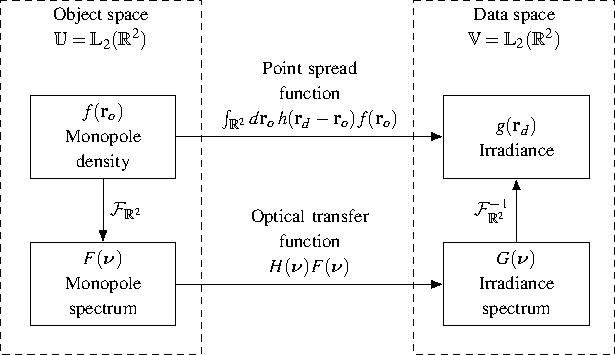
\includegraphics[scale=1.0]{../figures/monopole-block/monopole-block.pdf}
  \caption{
    The mapping between the object and data space of a monopole fluorescence microscope can be computed in two different bases---a delta function basis and a complex exponential basis. The change of basis can be computed with $n$-dimensional Fourier transforms denoted $\mathcal{F}_{\mbb{R}^n}$. Gray highlighting indicates which part of each expression is being named.
  }
  \label{fig:monopole-block}
\end{figure}

\subsubsection{Monopole coherent transfer functions}
\begin{align}
  |c(\rd - \roperp, \ropar)|^2 = h(\rd - \roperp, \ropar)
\end{align}
\begin{align}
  H(\bv) = \int_{\mbb{R}^3}d\bt\,C(\bt)C^*(\bt - \bv)
\end{align}
\begin{align}
  C(\bt) = \int_{\mbb{R}^3}d\bs{\mf{r}}\, c(\bs{\mf{r}})\,\text{exp}(-2\pi i\bs{\mf{r}}\cdot\bt).\label{eq:monoctf}
\end{align}
This implies that the three-dimensional coherent transfer function is a scaled pupil function on a spherical shell. 

\begin{figure}
  \centering
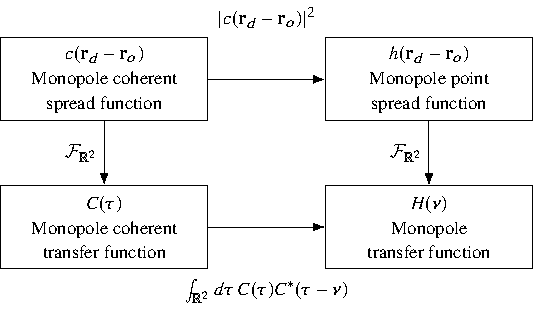
\includegraphics[scale=1.0]{../figures/monopole-transfer-functions/monopole-transfer-functions.pdf}
  \caption{
    The monopole transfer functions are related by a two-dimensional Fourier transform (right column). The coherent monopole transfer functions (left column) can be used to simplify the calculation of the remaining transfer functions.
  }
  \label{fig:monopole-transfer-functions}
\end{figure}

\subsubsection{Monopole pupil functions}
% First, consider the field created at $\rs$ by a monopole at $\ro$ 
% \begin{align}
%   U_s(\rs, \ro) \propto \frac{\text{exp}[2\pi i\nu_m|\rs - \ro|]}{|\rs - \ro|},
% \end{align}
% where $\nu_m = n_o/\lambda$. For monopoles near the origin we can find the fields on the Gaussian reference sphere of an objectives lens with focal length $f_0 \gg |\ro|$ by applying the approximation $|\rs - \ro| \approx |\rs| - \rs\cdot\ro/|\rs|$ and dropping second-order amplitude and constant phase terms
% \begin{align}
%   U_s(\rs, \ro) \propto \frac{1}{f_0}\text{exp}[-2\pi i\nu_m(\rs\cdot\ro)/f_0].
% \end{align}
% Next, we expand the coordinates into transverse and axial components
% \begin{align}
%   U_s(\rs, \ro) \propto \frac{1}{f_0}\text{exp}[-2\pi i\nu_m(\rsperp\cdot\roperp + \rspar\ropar)/f_0],
% \end{align}
% then rewrite in pupil coordinates using the relationships $\rsperp = \rpperp$ and $\rspar = \sqrt{f_0^2 - |\rppar|^2}$
% \begin{align}
%   U_p(\rpperp, \roperp, \ropar) \propto \frac{1}{f_0}\text{exp}\left[-2\pi i\nu_m\left(\rpperp\cdot\roperp + \rspar\sqrt{f_0^2 - |\roperp|^2}\right)/f_0\right].
% \end{align}
\add{Patrick: This section follows section 2A in the second paper \cite{chandler2019b} fairly closely with modifications for 3D.}

We can write the field in the pupil plane at point $\rpperp$ due to a monopole at $\ro = (\roperp, \ropar)$ as
\begin{align}
  U_p(\rpperp, \roperp, \ropar) \propto p_d(\rpperp, \ropar)\,\text{exp}\left[-2\pi i \frac{n_0}{\lambda f_0}\rpperp\cdot\roperp\right],
\end{align}
where $p_d(\rpperp, \ropar)$ is the \textit{defocused monopole pupil function}  
\begin{align}
  p_d(\rpperp, \ropar) = p(\rpperp)\, \text{exp}\left[-2\pi i\ropar\nu_m\sqrt{1 - (|\rpperp|/f_0)^2}\right],
\end{align}
and $p(\rpperp)$ is the usual pupil function which can be used to model angular cutoff, apodization, or aberrations.

Since the second lens is paraxial, we can model the relationship between the field in the pupil plane and the field on the detector with a scaled Fourier transform
\begin{align}
  U_d(\rd', \roperp, \ropar) \propto \int_{\mbb{R}^2}d\rpperp\,p_d(\rpperp, \ropar)\,\text{exp}\left[-2\pi i \frac{n_0}{\lambda f_0}\rpperp\cdot\roperp\right]\text{exp}\left[-2\pi i \frac{n_1}{\lambda f_1}\rpperp\cdot\rd'\right].
\end{align}

If we define $P(\btperp, \ropar)$ as the two-dimensional transverse Fourier transform of the defocused pupil function
\begin{align}
  P_d(\btperp, \ropar) = \int_{\mbb{R}^2}d\rpperp\, p_d(\rpperp, \ropar)\,\text{exp}(-2\pi i \rpperp\cdot\btperp),\label{eq:pupilF}
\end{align}
then we can rewrite the field on the detector as
\begin{align}
  U_d(\rd', \roperp, \ropar) \propto P\left(\frac{n_0}{\lambda f_0}\roperp + \frac{n_1}{\lambda f_1}\rd', \ropar\right).
\end{align}
After rewriting in terms of the magnification $m = -\frac{f_1 n_0}{f_0 n_1}$, demagnifying the coordinates with $\rd = \rd'/m$, and demagnifying the irradiance with $h(\rd - \roperp, \ropar) \propto h'(m[\rd - \roperp], \ropar) $, we find the defocused monopole point spread function is related to the Fourier transform of the defocused monopole pupil function by 
\begin{align}
  h(\rd-\roperp, \ropar) \propto \left|P\left(-\frac{n_0}{\lambda f_0}[\rd - \roperp], \ropar\right)\right|^2.
\end{align}
The monopole point spread function is the absolute square of the monopole coherent spread function so
\begin{align}
  c(\rd - \roperp, \ropar) \propto P\left(-\frac{n_0}{\lambda f_0}[\rd - \roperp], \ropar\right). \label{eq:monocsf}
\end{align}
Our final task is to calculate the monopole coherent transfer function by plugging Eq. \eqref{eq:monocsf} into Eq. \eqref{eq:monoctf} which yields
\begin{align}
  C(\bt) = \int_{\mbb{R}}dr^{\mypar}\int_{\mbb{R}^2}d\mb{r}^{\bot}\, P\left(-\frac{n_0}{\lambda f_0}\mb{r}^{\bot}, r^{\mypar}\right)\,\text{exp}(-2\pi i[\mb{r}^{\bot}\cdot\btperp + r^{\mypar}\btpar]).
\end{align}
Using Eq. \eqref{eq:pupilF} to simplify the transverse integral yields
\begin{align}
  C(\bt) \propto p\left(\frac{\lambda f_0}{n_0}\btperp\right) \int_{\mbb{R}}d r^{\mypar} \,\text{exp}\left(-2\pi i r^{\mypar}\sqrt{\nu_m - |\btperp|^2}\right)\,\text{exp}(-2\pi i r^{\mypar}\btpar)
\end{align}
Finally, we use the Fourier shift theorem to evaluate the axial integral to find that 
\begin{align}
  C(\bt) \propto p\left(\frac{\lambda f_0}{n_0}\btperp\right)\,\delta\left(\btpar - \sqrt{\nu_m^2 - |\btperp|^2}\right).\label{eq:monoctf}
\end{align}

% \subsection{Three-dimensional dipole transfer functions}
% \subsubsection{Dipole transfer functions}
% \begin{figure}
%   \hspace{-6em}
%   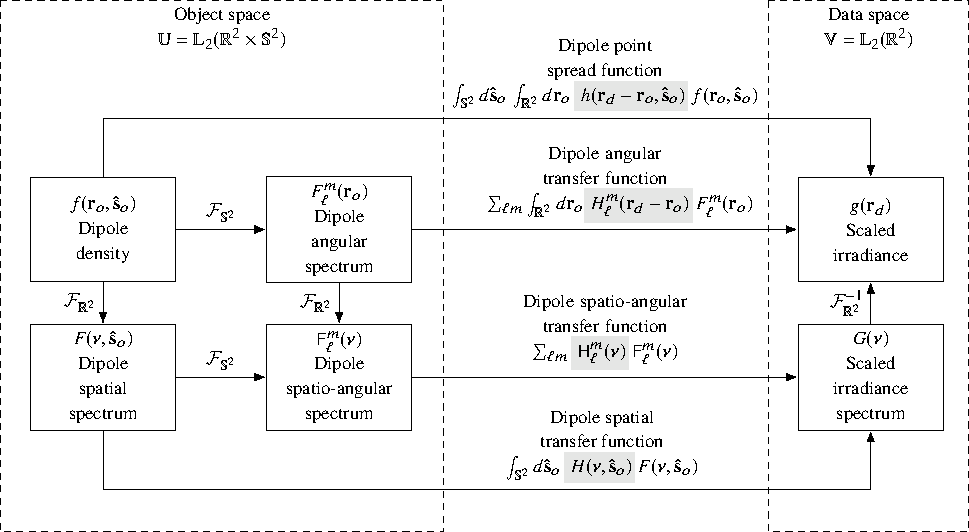
\includegraphics[scale=1.0]{../figures/dipole-block/dipole-block.pdf}
%   \caption{
%     % The mapping between the object space and data space of a dipole imaging system can be computed in four different bases---a delta function basis, a complex-exponential/angular-delta basis, a spatial-delta/spherical-harmonic basis, and a complex-exponential/spherical-harmonic basis. The changes of basis can be computed with the two-dimensional Fourier transform denoted $\mathcal{F}_{\mbb{R}^2}$, and the spherical Fourier transform denoted $\mathcal{F}_{\mbb{S}^2}$. Gray highlighting indicates which part of each expression is being named.
%   }
%   \label{fig:dipole-block}      
% \end{figure}

% \subsubsection{Dipole coherent transfer functions}

% \begin{figure}
%   \hspace{-2em}
% \includegraphics[scale=1.0]{../figures/dipole-transfer-functions/dipole-transfer-functions.pdf}
% \caption{
%   % There is one transfer function for each set of object-space basis functions, and these transfer functions are related by two-dimensional and spherical Fourier transforms---see center and right columns. There is an additional pair of coherent transfer functions that are useful for calculating the transfer functions---see left column.
% }
%   \label{fig:transfer-functions}
% \end{figure}

% \subsubsection{Dipole pupil functions}

\section{Results}
\subsection{Monopole transfer functions}
We can model an aplanatic microscope imaging monopole emitters with the scalar pupil function
\begin{align}
  p(\rpperp) \propto  \tilde{C}\left(\frac{|\rpperp|}{f_0}\right)\Pi\left(\frac{|\rpperp|}{2f_0\sin\alpha}\right). \label{eq:monopupil}
\end{align}

Plugging Eq. \eqref{eq:monopupil} in Eq. \eqref{eq:monoctf} yields
\begin{align}
  C(\bt) \propto \tilde{C}\left(\frac{|\btperp|}{\nu_m}\right)\,\delta\left(\btpar - \sqrt{\nu_m^2 - |\btperp|^2}\right)\,\Pi\left(\frac{|\btperp|}{\nu_c}\right)
\end{align}
where $\nu_c = 2\text{NA}/\lambda$, $\text{NA} = n_0\sin\alpha$, and 
\begin{align}
  \tilde{C}(x) = (1 - x^2)^{-1/4}.
\end{align}

\add{To make the units check we need to add a normalization factor of $\frac{1}{\nu_c}$ to the coherent transfer function. Arguably this factor should have been included in the Eqs. 22 and 23 of the second paper \cite{chandler2019b}, but we played a bit loose with the proportionality symbol. I'm not sure if there's a more elegant way to motivate this factor of $\frac{1}{\nu_c}$.}
\begin{align}
  C(\bt) \propto \frac{1}{\nu_c}\tilde{C}\left(\frac{|\btperp|}{\nu_m}\right)\,\delta\left(\btpar - \sqrt{\nu_m^2 - |\btperp|^2}\right)\,\Pi\left(\frac{|\btperp|}{\nu_c}\right)
\end{align}

In Appendix \ref{sec:monoauto} we calculate the autocorrelation of the coherent transfer function and show that the monopole transfer function is given by
\begin{align}
  H(\bv) = \delta(\bv) + \frac{4\tau_{\circ}^2\bvpar}{\pi\nu_c^2|\bv|\nu_m}\sqrt{p^2 - 1}\,E\left(\beta_m, \frac{p}{\sqrt{p^2 - 1}}\right),
\end{align}
where $E(\beta_m, k)  = \int_0^{\beta_m} d\phi\sqrt{1 - k^2\sin^2\phi}$ is an incomplete elliptic integral of the second kind and
\begin{align}
  p = \frac{|\bvperp|\nu_\circ}{\bvpar|\bv|},\qquad
  \nu_\circ = \sqrt{\nu_m^2 - (|\bv|/2)^2},\qquad
  \beta_m = \cos^{-1}\left(\frac{1}{p}\left[\frac{2\nu_m}{|\bvpar|}\cos\alpha + 1\right]\right).
\end{align}

We can also investigate the three-dimensional monopole transfer functions under the paraxial approximation by expanding the coherent transfer about $|\btperp| = 0$ and dropping second-order terms
\begin{align}
  C(\bt) \propp \frac{1}{\nu_c}\delta\left(\btpar - \nu_m + |\btperp|^2/2\nu_m\right)\,\Pi\left(\frac{|\btperp|}{\nu_c}\right).
\end{align}
In Appendix B we calculate the autocorrelation of the paraxial coherent transfer and show that the paraxial monopole transfer function is given by
\begin{align}
  H(\bv) \eqp \delta(\bv) + \frac{8\nu_m}{\pi\nu_c^2}\text{nez}\left(\frac{|\bvperp|}{\nu_c}, \frac{2\nu_m|\bvpar|}{\nu_c^2}\right),
\end{align}
where
\begin{align}
 \text{nez}(x, z) = \frac{1}{2|x|}\text{Re}\left[\sqrt{1 - \left(\frac{|z|}{|x|} + |x|\right)^2}\right].
\end{align}

% \subsection{Dipole transfer functions}
% \subsubsection{Dipole point spread function}

% \subsubsection{Dipole spatial transfer function}

% \subsubsection{Dipole angular transfer function}

% \subsubsection{Dipole spatio-angular transfer function}

\section{Discussion}
% Dipole phase masking:
% Azimuthal polarization filtering: \cite{lew2014}
% Metasurface polarization filtering: \cite{backlund2016}

\section{Conclusions}

\section*{Funding}
National Institute of Health (NIH) (R01GM114274, R01EB017293).

\section*{Acknowledgments}
TC was supported by a University of Chicago Biological Sciences Division Graduate Fellowship, and PL was supported by a Marine Biological Laboratory Whitman Center Fellowship. Support for this work was provided by the Intramural Research Programs of the National Institute of Biomedical Imaging and Bioengineering. 

\section*{Disclosures}
The authors declare that there are no conflicts of interest related to this article.

\bibliography{/Users/Talon/Library/texmf/talon}
\appendix

\section{Multidimensional curvilinear delta functions}

\add{TODO: Summarize operational rules for tricky curvilinear delta functions. TBH I haven't mastered these rules yet.}
% In this appendix we review operational rules for manipulating multidimensional curvilinear delta functions. For a gentle introduction see Bracewell \cite{bracewell2004} and for details see Gelfand and Shilov \cite{gelfand2016}. Here we attempt to be brief and accessible.

% $\delta(f(x))$

% $\delta(f(\mb{r}))$

% $\delta(\mb{f}(\mb{r}))$

\section{Three-dimensional monopole transfer functions}\label{sec:monoauto}
\add{I have recently reworked this section with units in mind, and as far as I can tell all of the units are consistent. The paraxial results agree with the literature and when they project to 2D we get a result that is consistent with the previous paper.}

\add{I'm still having problems with the high-NA result, though. When I integrate over the axial coordinate the result is not normalized (see Fig. \ref{fig:compare}), and the result does not agree with Sheppard/Barakat \cite{barakat1963, sheppard1994} who predict a suppressed low-frequency response and an enhanced high-frequency response for high-NA objectives compared to the paraxial approximation. I'm hot on the trail of a few issues, but I'd appreciate any flags.}

In this appendix we will calculate the three-dimensional monopole transfer function
by evaluating the integral
\begin{align}
  H(\bv) = \int_{\mbb{R}^3}d\bt\, C(\bt + \bv/2)\,C^*(\bt - \bv/2). \label{eq:3dauto}
\end{align}
We will start by calculating the transfer function for the most general high-aperture case by setting the coherent transfer function to
\begin{align}
  C(\bt) \propto \frac{1}{\nu_c}\tilde{C}\left(\frac{|\btperp|}{\nu_m}\right)\,\delta\left(\btpar - \sqrt{\nu_m^2 - |\btperp|^2}\right)\,\Pi\left(\frac{|\btperp|}{\nu_c}\right).
\end{align}
Equivalently, we can express the high-aperture coherent transfer function in spherical coordinates as
\begin{align}
  C(\bt) \propto \,\frac{1}{\nu_c}\sqrt{\cos\theta_{\tau}}\,\delta\left(|\bt| - \nu_m\right)\,\Pi\left(\frac{\theta_{\tau}}{2\alpha}\right).
\end{align}
Therefore, we can interpret the integral in Eq. \eqref{eq:3dauto} as the autocorrelation of a $\sqrt{\cos\tau_\theta}$-weighted spherical cap with radius $\nu_m$ and half angle $\alpha$.

For $|\bv| = 0$ we can integrate over the spherical cap to find that 
\begin{align}
  H(\bv) \propto \frac{1}{\nu_c^2}\int_{0}^{\infty}|\bt|^2d|\bt|\int_0^{2\pi}d\phi_\tau\int_{0}^{\alpha}d\theta_\tau \sin\theta_\tau\cos\theta_\tau\delta(|\bt| - \nu_m)\delta(|\bt| - \nu_m) = \frac{\pi}{4}\delta(|\bv|).
\end{align}

When $|\bv| > 0$ we need to integrate over the intersection of the two spherical
caps which only intersect when
\begin{align}
  |\bvpar| < \sqrt{\nu_m^2 - (|\bvperp| - \nu_m\sin\alpha)^2} - \nu_m\cos\alpha. 
\end{align}
Therefore, the transfer function is zero when this condition is not satisfied.

\begin{figure}
  \centering
  \includegraphics[scale=0.3]{../figures/caps/general.pdf}
  \includegraphics[scale=0.25]{../figures/caps/spherical.pdf}\hspace{0.5em}
  \includegraphics[scale=0.28]{../figures/caps/cylindrical.pdf}
  \caption{Geometric constructions and coordinate systems for performing the three-dimensional autocorrelation. (Top) Two spherical caps with spherical radius $\nu_m = n_o/\lambda$ and base diameter $\nu_c = 2\text{NA}/\lambda$ are shifted by $\bv$ and intersect along a circular arc in the plane perpendicular to $\bv$. (Bottom left) We define a spherical coordinate system for each cap. These coordinate systems  are most convenient for expressing the individual coherent transfer functions. (Bottom right) We define a cylindrical coordinate system with the long axis of the cylinder parallel to the shift direction $\bv$ and the azimuthal angle $\beta_\tau$ defined with respect to the lowest point of each cylindrical slice. This coordinate system is most convenient for integrating over the circular arc of intersection.}
  \label{fig:caps}
\end{figure}

By inspection of Fig. \ref{fig:caps}, the intersection of the two shifted spherical caps is a circular arc centered on the origin in the plane perpendicular to the shift direction $\bv$. To integrate along this arc it will be convenient to define three new coordinate systems: (1, 2) two spherical coordinate systems defined with respect to the centers of the shifted spheres, and (3) a cylindrical coordinate system with long axis parallel to the shift direction $\bv$. The shifted spherical coordinate systems are straightforward to derive as
\begin{align}
  \begin{bmatrix}
    \tau_x\\
    \tau_y\\
    \btpar
  \end{bmatrix}
  =
  \begin{bmatrix}
    |\bt|_{1,2}\sin\theta_{\tau_{1,2}}\cos\phi_{\tau_{1,2}} \pm \nu_x/2\\
    |\bt|_{1,2}\sin\theta_{\tau_{1,2}}\sin\phi_{\tau_{1,2}} \pm \nu_y/2\\
    |\bt|_{1,2}\cos\theta_{\tau_{1,2}} \pm \bvpar/2
  \end{bmatrix},\label{eq:spherical}
\end{align}
where the subscripts and $\pm$ indicate which of the pair of shifted coordinate systems we are using.

Deriving the cylindrical coordinate system is more involved. We follow Arnison and Sheppard \cite{arnison2002} and define a cylindrical coordinate system for shifts along the $x$ axis $\bv = (1,0,0)$ then generalize to arbitrary shifts by multiplying with rotation matrices
\begin{align}
  \begin{bmatrix}
    \tau_x\\
    \tau_y\\
    \btpar
  \end{bmatrix}
  &= \mb{R}_{\mb{z}}(-\tan^{-1}(\nu_y/\nu_x)\mb{R}_{\mb{y}}(\sin^{-1}(\bvpar/|\bv|))
  \begin{bmatrix}
    \tau_\xi\\
    \tau_R\sin\beta_\tau\\
    -\tau_R\cos\beta_\tau
  \end{bmatrix}\nonumber\\
  &=
  \begin{bmatrix}
    \displaystyle\frac{\nu_x}{|\bv|}\tau_\xi + \frac{\tau_R}{|\bvperp||\bv|}(\bvpar\nu_x\cos\beta_\tau - |\bv|\nu_y\sin\beta_\tau)\\[1em]
    \displaystyle\frac{\nu_y}{|\bv|}\tau_\xi + \frac{\tau_R}{|\bvperp||\bv|}(\bvpar\nu_y\cos\beta_\tau + |\bv|\nu_x\sin\beta_\tau)\\[1em]
    \displaystyle\frac{\bvpar}{|\bv|}\tau_\xi - \frac{|\bvperp|\tau_R}{|\bv|}\cos\beta_\tau
  \end{bmatrix},\label{eq:cylindrical}
\end{align}
where
\begin{align}
  \mb{R}_\mb{z}(\theta) =
  \begin{bmatrix}
    \cos\theta & 0 & -\sin\theta\\
    0 & 1 & 0\\
    \sin\theta & 0 &\cos\theta
  \end{bmatrix}\, ,\quad 
  \mb{R}_\mb{y}(\theta) =
  \begin{bmatrix}
    \cos\theta & \sin\theta & 0\\
    -\sin\theta & \cos\theta & 0\\
    0 & 0 & 1
  \end{bmatrix}.
\end{align}

To evaluate the integral we need to express it in our new cylindrical coordinate system. We start by considering the pair of delta functions in the integrand $\delta(|\bt - \bv/2| - \nu_m)\,\delta(|\bt + \bv/2| - \nu_m)$. The spherical shells intersect in a circle of radius $\nu_\circ = \sqrt{\nu_m^2 - (|\bv|/2)^2}$ centered on the origin so we expect the delta functions to become $\delta(\tau_\xi)\,\delta(\tau_R - \nu_\circ)$ in the cylindrical coordinate system. However, we need to preserve the ``strength'' of the delta functions in the new coordinate system (see Bracewell \cite{bracewell2004} for operational rules and see Gelfand and Shilov \cite{gelfand2016} for a detailed discussion), so we normalize by the Jacobian determinant in each coordinate system. After accounting for the changing strength of the delta functions we find that
\begin{align}
  \delta(|\bt - \bv/2| - \nu_m)\,\delta(|\bt + \bv/2| - \nu_m) = \frac{\nu_\circ}{|\bv|}\delta(\tau_\xi)\,\delta(\tau_R - \nu_\circ).
\end{align}
\add{This step is a prime candidate for an error. I derived this factor
  $\frac{\nu_\circ}{|\bv|}$ by matching the Jacobian on both sides, but this
  disagrees with the factor Arnison \cite{arnison2002} uses which is $\propto \frac{1}{|\bv|\nu_\circ}$. Arnison's factor doesn't seem to have the correct units...although all of the Sheppard papers seem pretty free-form when it comes to normalizing/units.}

The integrating measure in the cylindrical coordinate system is
\begin{align}
  d\bt = \tau_R d\tau_R d\tau_\xi d\beta_\tau,
\end{align}
so we can write the integral as 
\begin{align}
  H(\bv) \propto \frac{1}{\nu_c^2}\frac{\nu_\circ}{|\bv|}\int_{\mbb{R}}d\tau_\xi\int_{0}^{\infty}\tau_Rd\tau_R\int_{-\pi}^{\pi}d\beta_\tau\, \sqrt{\cos\tau_{\theta_1}\cos\tau_{\theta_2}}\,\delta(\tau_\xi)\delta(\tau_R - \nu_\circ)\,\Pi\left(\frac{\tau_{\theta_1}}{2\alpha}\right)\Pi\left(\frac{\tau_{\theta_2}}{2\alpha}\right).
\end{align}

Next, we express the integrand in cylindrical coordinates. Equating the $\btpar$ components in Eqs. \eqref{eq:spherical} and \eqref{eq:cylindrical} and evaluating on the circle of intersection ($|\bt|\rightarrow \nu_m$, $\tau_\xi\rightarrow 0$, $\tau_R\rightarrow \nu_\circ$) yields the relationship
\begin{align}
  \nu_m\cos\theta_{\tau_{1,2}} \pm \frac{\bvpar}{2} = -\frac{|\bvperp|\nu_\circ}{|\bv|}\cos\beta_\tau\label{eq:angles}.
\end{align}
The integrand is written in terms of $\cos\tau_{\theta_{1,2}}$, so we rewrite Eq. \eqref{eq:angles} to find the relationship
\begin{align}
  \cos\theta_{\tau_{1,2}} = \frac{1}{\nu_m}\left(-\frac{|\bvperp|\nu_\circ}{|\bv|}\cos\beta_\tau\mp \frac{\bvpar}{2}\right) = \frac{\bvpar}{2\nu_m}\left(-p\cos\beta_\tau \mp 1\right)
\end{align}
where
\begin{align}
  p = \frac{2|\bvperp|\nu_\circ}{\bvpar|\bv|}.
\end{align}

We can also use Eq. \eqref{eq:angles} to find the limits of integration for $\tau_\beta$ by setting $\tau_{\theta_2} \rightarrow \alpha$ then solving for $\tau_\beta$ to find the maximum azimuthal angle $\beta_m$
\begin{align}
  \beta_m = \cos^{-1}\left[\frac{1}{p}\left(\frac{2\nu_m}{|\bvpar|}\cos\alpha + 1\right)\right].
\end{align}

Bringing everything together yields the one-dimensional integral
\begin{align}
  H(\bv) \propto \frac{\nu_\circ^2\bvpar}{2\nu_c^2|\bv|\nu_m}\int_{-\beta_m}^{\beta_m}d\tau_\beta\, \sqrt{p^2\cos^2\beta_\tau - 1}, 
\end{align}
which can be written as 
\begin{align}
  H(\bv) \propto \frac{\tau_{\circ}^2\bvpar}{\nu_c^2|\bv|\nu_m}\sqrt{p^2 - 1}\,E\left(\beta_m, \frac{p}{\sqrt{p^2 - 1}}\right),
\end{align}
where $E(\beta_m, k)  = \int_0^{\beta_m} d\phi\sqrt{1 - k^2\sin^2\phi}$ is an incomplete elliptic integral of the second kind.

After normalization, the complete transfer function is given by
\begin{align}
  H(\bv) = \delta(|\bv|) + \frac{4\tau_{\circ}^2\bvpar}{\pi\nu_c^2|\bv|\nu_m}\sqrt{p^2 - 1}\,E\left(\beta_m, \frac{p}{\sqrt{p^2 - 1}}\right).
\end{align}

Next, we calculate the monopole transfer function under the paraxial approximation. We approximate the $\sqrt{\cos\theta_\tau}$-weighted spherical cap with a truncated paraboloid
\begin{align}
  C(\bt) \propp \frac{1}{\nu_c}\delta\left(\btpar - \nu_m + |\btperp|^2/2\nu_m\right)\,\Pi\left(\frac{|\btperp|}{\nu_c}\right). \label{eq:ctf}
\end{align}

For the high-aperture case we evaluated the three-dimensional autocorrelation
directly, but for the paraxial case it is easier to evaluate the two-dimensional
autocorrelation of the defocused coherent transfer functions. We rewrite the
three-dimensional transfer function as
\begin{align}
  H(\bv) = \int_{\mbb{R}}dr^{\mypar}\,H^{(d)}(\bvperp,r^{\mypar})\,\text{exp}(-2\pi i r^{\mypar}\bvpar),\label{eq:def3dtf}
\end{align}
where $H^{(d)}(\bvperp,r^{\mypar})$ is the defocused transfer function given by
\begin{align}
  H^{(d)}(\bvperp,r^{\mypar}) = \int_{\mbb{R}^2}d\btperp\,C^{(d)}(\btperp + \bvperp/2, r^{\mypar})C^{(d)*}(\btperp - \bvperp/2, r^{\mypar}), \label{eq:defautocorr}
\end{align}
and $C^{(d)}(\btperp, r^{\mypar})$ is the defocused coherent transfer function given by
\begin{align}
  C^{(d)}(\btperp, r^{\mypar}) = \int_{\mbb{R}}d\btpar\, C(\bt)\,\text{exp}(2\pi i r^{\mypar}\btpar).\label{eq:deftf}
\end{align}
We plug Eq. \eqref{eq:ctf} into Eq. \eqref{eq:deftf} and evaluate the Fourier transform to find that the defocused coherent transfer function is
\begin{align}
  C^{(d)}(\btperp, r^{\mypar}) \propp \frac{1}{\nu_c}\text{exp}(2\pi i r^{\mypar}[-\nu_m + |\btperp|^2/2\nu_m])\Pi\left(\frac{|\btperp|}{\nu_c}\right), \label{eq:defctf}
\end{align}
which we can interpret as a disk with uniform magnitude and quadratic phase factor that depends on the defocus $r^{\mypar}$. 

To evaluate the three-dimensional transfer function at $|\bv| = 0$ we start by evaluating the defocused transfer function at $|\bvperp| = 0$
\begin{align}
  H^{(d)}(\bv, r^{\mypar}) = \frac{\pi}{4}. \label{eq:result}
\end{align}
After plugging \eqref{eq:result} into Eq. \eqref{eq:def3dtf} and evaluating the Fourier transform we find that 
\begin{align}
  H(\bv) = \frac{\pi}{4}\delta(|\bv|). 
\end{align}

When $|\bv| > 0$ we need to integrate over the intersection of the two truncated paraboloids which only intersect when
\begin{align}
  |\bvpar| < -\frac{1}{2\nu_m}|\bvperp|(|\bvperp| - \nu_c). 
\end{align}
Therefore, the paraxial transfer function is zero when this condition is not satisfied.

First we evaluate the defocused transfer function by plugging Eq. \eqref{eq:defctf} into Eq. \eqref{eq:defautocorr}
\begin{align}
  H^{(d)}(\bvperp,r^{\mypar}) \propp \frac{1}{\nu_c^2}\int_{\mbb{R}^2}d\btperp\, \text{exp}(2\pi i r^{\mypar}[|\btperp + \bvperp/2|^2/2\nu_m])\, \text{exp}(-2\pi i r^{\mypar}[|\btperp - \bvperp/2|^2/2\nu_m])\nonumber\\\Pi\left(\frac{|\btperp + \bvperp/2|}{\nu_c}\right) \Pi\left(\frac{|\btperp - \bvperp/2|}{\nu_c}\right),
\end{align}
then simplifying the complex exponentials
\begin{align}
  H^{(d)}(\bvperp,r^{\mypar}) \propp \frac{1}{\nu_c^2}\int_{\mbb{R}^2}d\btperp\, \text{exp}(2\pi i r^{\mypar}[\btperp\cdot\bvperp/\nu_m])\Pi\left(\frac{|\btperp + \bvperp/2|}{\nu_c}\right) \Pi\left(\frac{|\btperp - \bvperp/2|}{\nu_c}\right).\label{eq:defocusresult}
\end{align}
Next, we plug Eq. \eqref{eq:defocusresult} into Eq. \eqref{eq:def3dtf} and evaluate the
Fourier transform to find that 
\begin{align}
  H(\bv) \propp \frac{1}{\nu_c^2}\int_{\mbb{R}^2}d\btperp\, \delta(\bvpar - \btperp\cdot\bvperp/\nu_m)\Pi\left(\frac{|\btperp + \bvperp/2|}{\nu_c}\right) \Pi\left(\frac{|\btperp - \bvperp/2|}{\nu_c}\right).
\end{align}
\begin{figure}
  \centering
  \includegraphics[scale=0.2]{../figures/para-geometry/para-geometry.pdf}
  \caption{Geometric construction for evaluating the three-dimensional autocorrelation under the paraxial approximation. We need to integrate over a line perpendicular to the transverse shift direction $\bvperp$ that is displaced from the origin by $\nu_m|\bvpar|/|\bvperp|$ and truncated by the shifted circles with diameter $\nu_c$.}
  \label{fig:geometry}
\end{figure}

We can evaluate this integral with the help of the geometric construction in Fig. \ref{fig:geometry}. The delta function corresponds to a line perpendicular to the transverse shift direction $\bvperp$ displaced from the origin by $\nu_m|\bvpar|/|\bvperp|$. Within the intersection of the shifted circles this line has length $2\sqrt{(\nu_c/2)^2 - ([\nu_m|\bvpar|/|\bvperp|] + [|\bvperp|/2])^2}$. Finally, the ``strength'' of the delta function is $\nu_m/|\bvperp|$, so the integral evaluates to 
\begin{align}
  H(\bv) \propp \frac{2\nu_m}{\nu_c^2|\bvperp|}\sqrt{\left(\frac{\nu_c}{2}\right)^2 - \left(\frac{\nu_m|\bvpar|}{|\bvperp|} + \frac{|\bvperp|}{2}\right)^2}. 
\end{align}

After normalization, the complete paraxial transfer function is 
\begin{align}
  H(\bv) \eqp \delta(|\bv|) + \frac{8\nu_m}{\pi\nu_c^2|\bvperp|}\text{Re}\left\{\sqrt{\left(\frac{\nu_c}{2}\right)^2 - \left(\frac{\nu_m|\bvpar|}{|\bvperp|} + \frac{|\bvperp|}{2}\right)^2}\right\}.
\end{align}

We can rewrite the paraxial transfer function in a scaled form 
\begin{align}
  H(\bv) \eqp \delta(|\bv|) + \frac{8\nu_m}{\pi\nu_c^2}\text{nez}\left(\frac{|\bvperp|}{\nu_c}, \frac{2\nu_m|\bvpar|}{\nu_c^2}\right),
\end{align}
where we have defined the function
\begin{align}
 \text{nez}(x, z) = \frac{1}{2|x|}\text{Re}\left[\sqrt{1 - \left(\frac{|z|}{|x|} + |x|\right)^2}\right]
\end{align}
and named it for its resemblance to pince-nez (nose-pinching glasses)---see Fig. \ref{fig:nez}.
\begin{figure}
  \centering
  \includegraphics[scale=0.9]{../figures/nez/nez.pdf}
  \caption{Plot of $\text{nez}(x,z)$ with contours on integer values between 0 and 5. $\text{nez}(x,z)$ has a singularity at the origin, so we have truncated values above 10.}
  \label{fig:nez}
\end{figure}

We can recover the two-dimensional paraxial transfer function by integrating over the axial coordinate
\begin{align}
  H(\bvperp) \eqp \int_{\mbb{R}}d\bvpar\, H(\bv) = \frac{4}{\pi}\text{chat}_0\left(\frac{|\bvperp|}{\nu_c}\right), 
\end{align}
where we have used
\begin{align}
  \int_{\mbb{R}}dz\,\text{nez}(x,z) = \text{chat}_0(x) = \frac{1}{2}\left[\cos^{-1}|x| - |x|\sqrt{1-x^2}\right]\Pi\left(\frac{x}{2}\right).
\end{align}

\begin{figure}
  \centering
  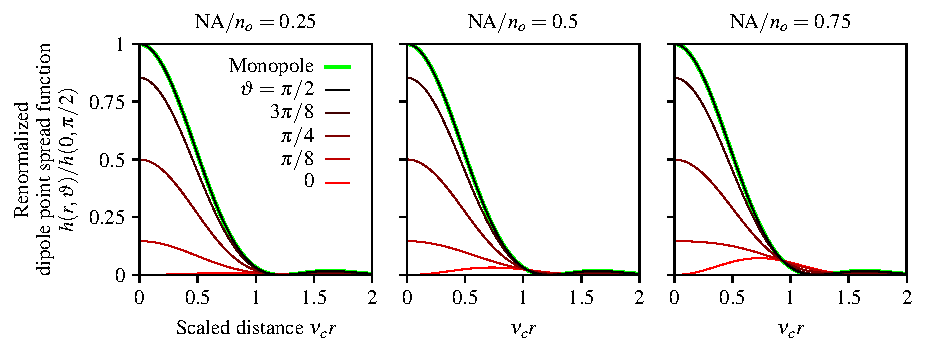
\includegraphics[scale=0.85]{../figures/monopole-psf/dpsf.pdf}
  \caption{Comparison of high-aperture and paraxial three-dimensional transfer functions for $\text{NA} = (1.00, 1.25, 1.50)$, $n_o = 1.5$, and $\lambda = 500\,\text{nm}$. \add{Notice the units: input spatial frequencies are in  m${}^{-1}$ and the output is in m${}^{+1}$. I have overlaid each plot with two lines: a blue line which is the paraxial transverse transfer function ($\text{chat}(\nu/\nu_c)$) and a green line which is the numerical integral of the 3D transfer function over $\bvpar$. The blue and green lines should have their own $y$ axis, but I'm reusing the left $y$ axis without units. In the paraxial case these lines agree which is a good check that my results are correct. In the high-aperture case the green line is not normalized, and I expect the green line to be lower than the blue line at low frequencies and higher than the blue line at high frequencies (see Barakat \cite{barakat1963}). Therefore, I'm searching for an error that makes the high-aperture transfer function too large everywhere (normalization) and too small at high-frequencies.}}
  \label{fig:compare}
\end{figure}



\end{document}
